\section{\isklearn pipeline composition per dataset}

Pipeline structures selected by \irace for each dataset are given as sunburst plots in Figure~\ref{fig:dataset_composition}.

\begin{figure*}
    \centering
    
  	\begin{subfigure}[t]{0.3\textwidth}
    \centering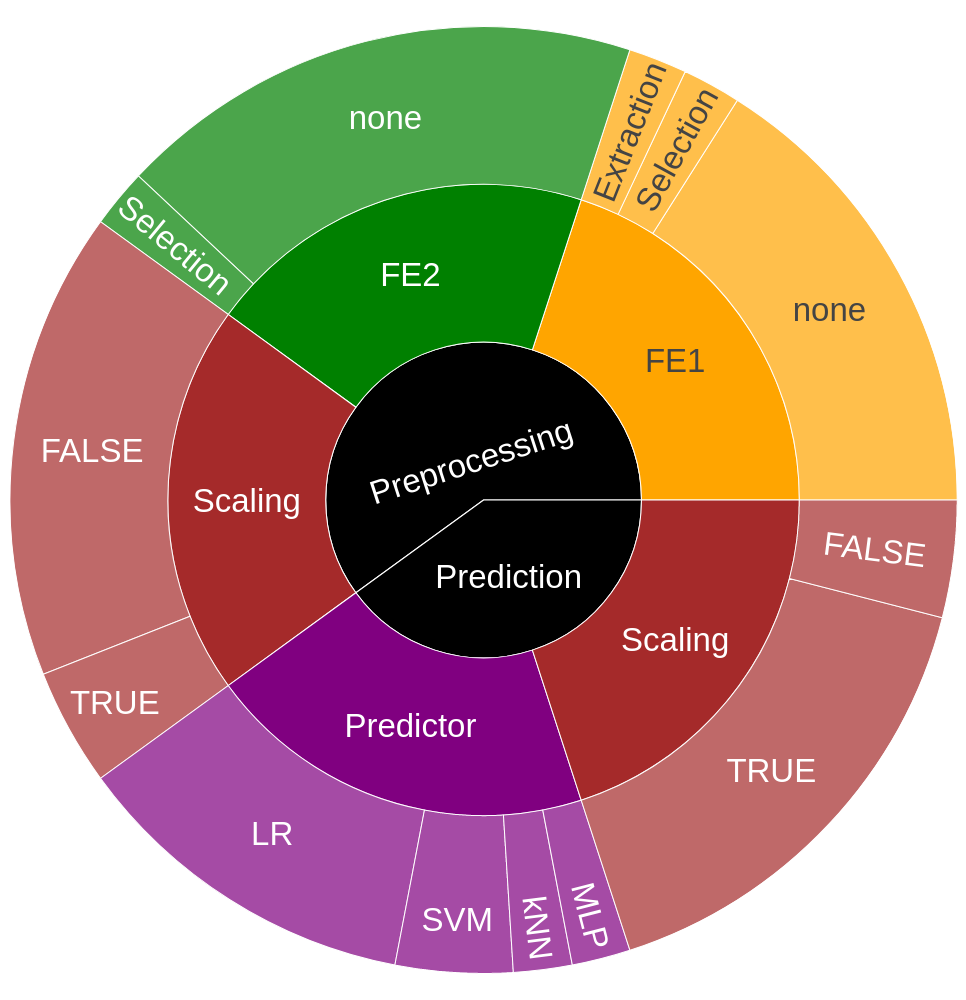
\includegraphics[width=0.9\textwidth]{img/sunburst/cifar10.png}
    \caption{CIFAR-10}
  	\end{subfigure}
  	\begin{subfigure}[t]{0.3\textwidth}
    \centering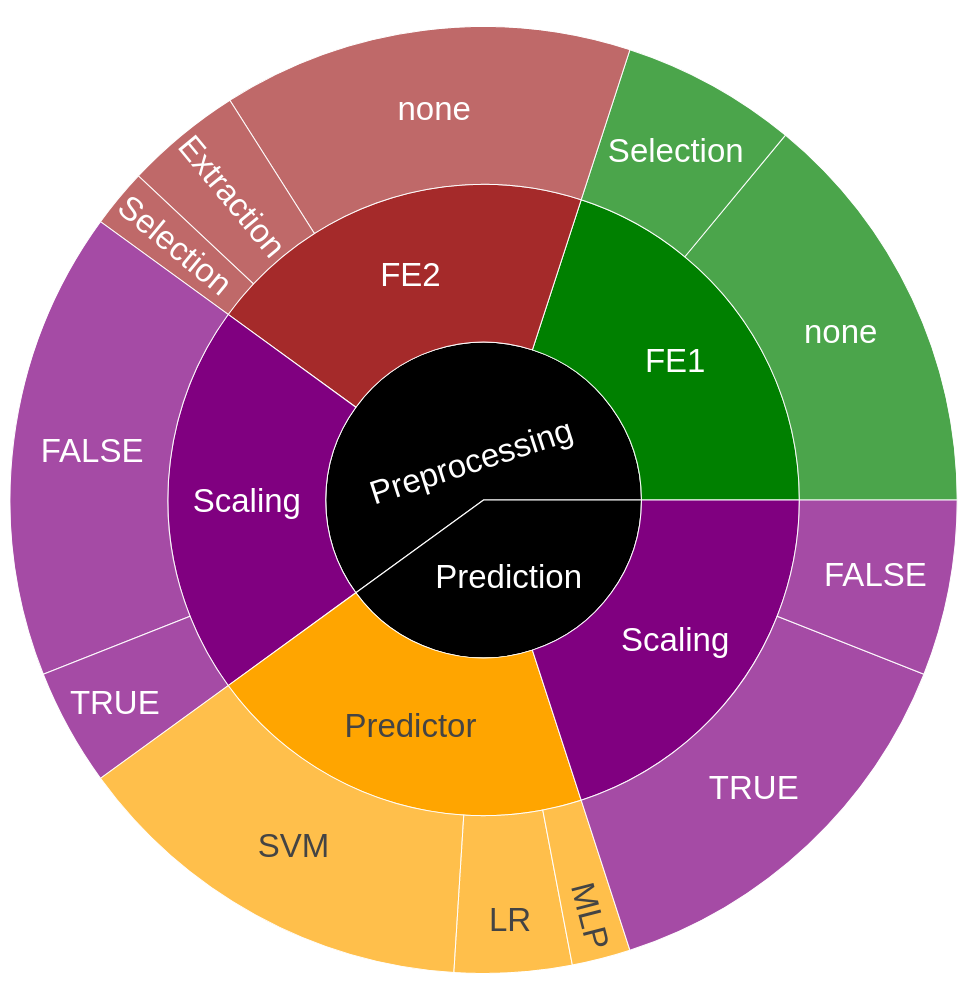
\includegraphics[width=0.9\textwidth]{img/sunburst/fmnist.png}
    \caption{FMNIST}
  	\end{subfigure}
	\begin{subfigure}[t]{0.3\textwidth}
    \centering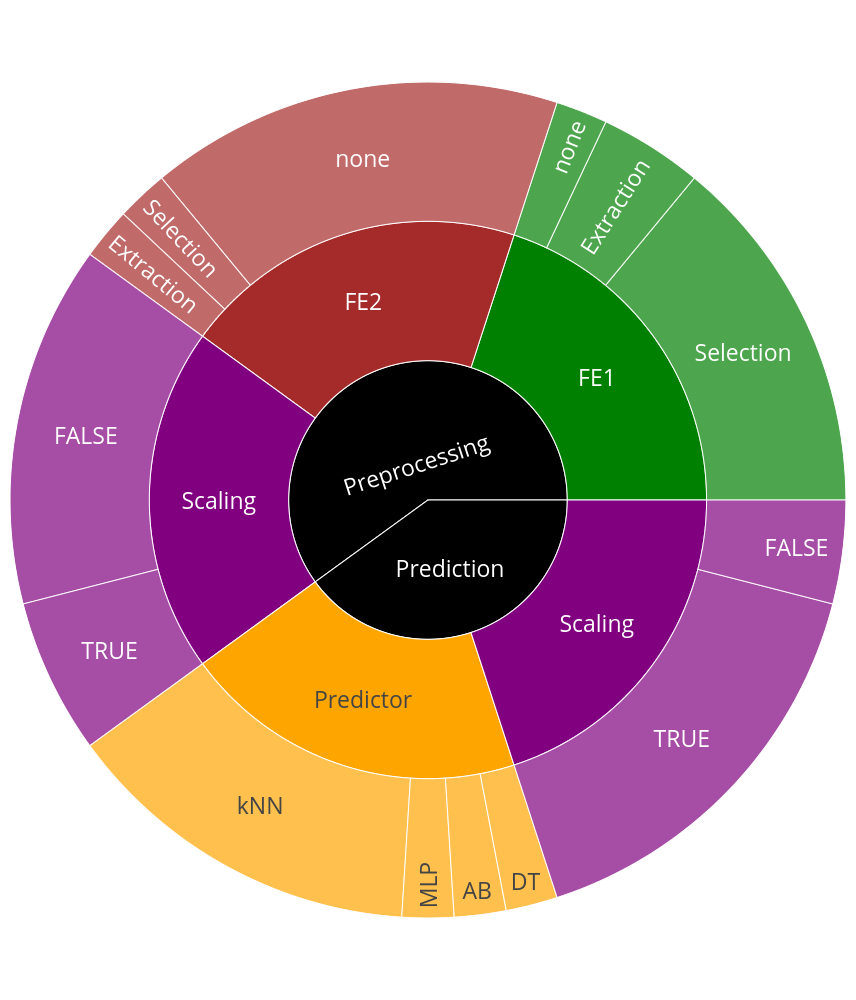
\includegraphics[width=0.9\textwidth]{img/sunburst/svhn.png}
    \caption{SVHN}
  	\end{subfigure}

  	\begin{subfigure}[t]{0.3\textwidth}
    \centering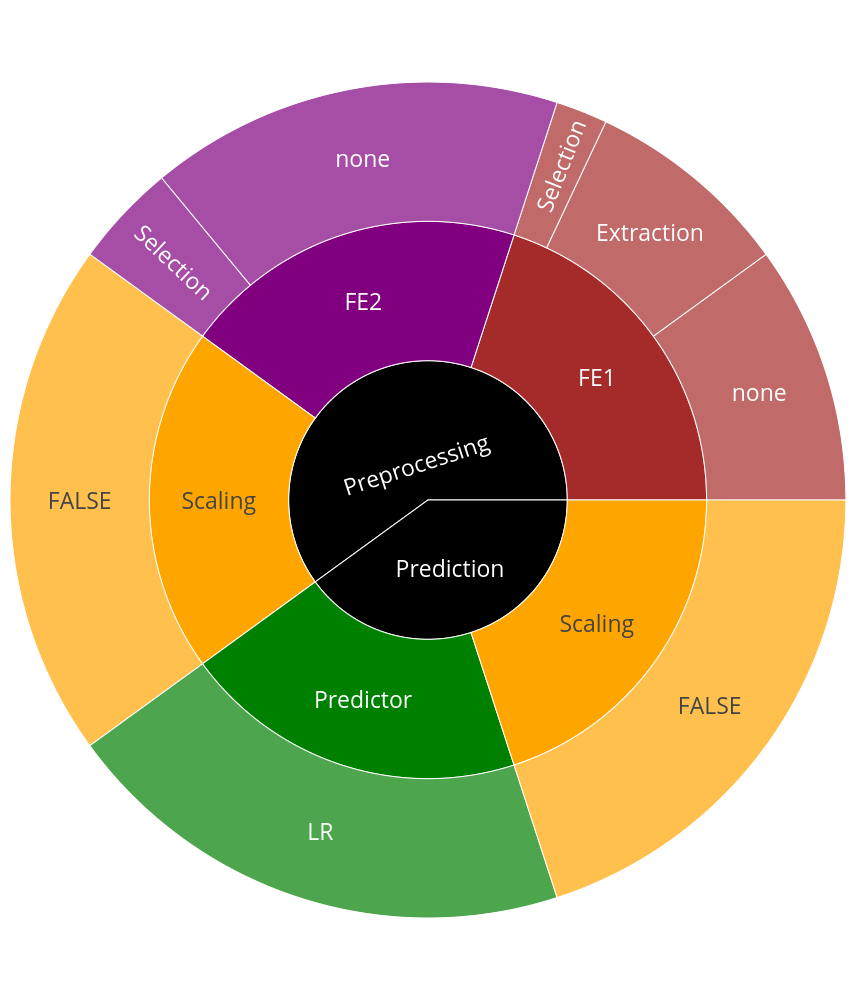
\includegraphics[width=0.9\textwidth]{img/sunburst/reuters.png}
    \caption{LMRD}
  	\end{subfigure}
  	\begin{subfigure}[t]{0.3\textwidth}
    \centering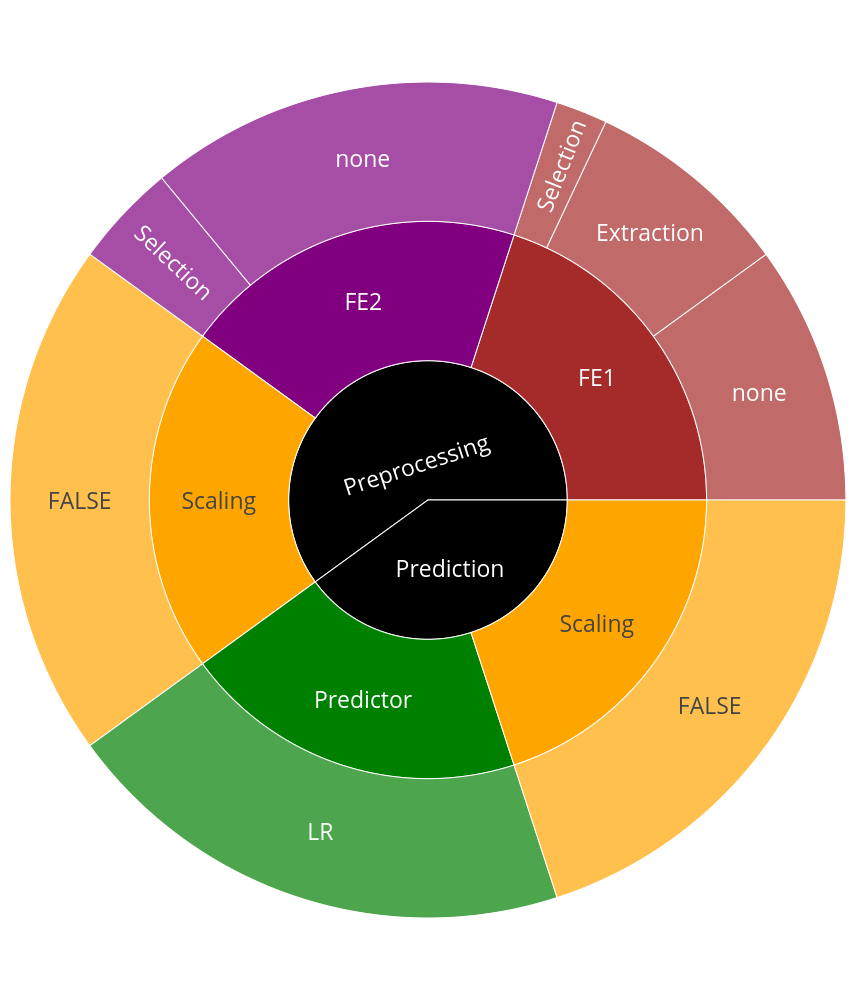
\includegraphics[width=0.9\textwidth]{img/sunburst/reuters.png}
    \caption{Reuters}
  	\end{subfigure}
	\begin{subfigure}[t]{0.3\textwidth}
    \centering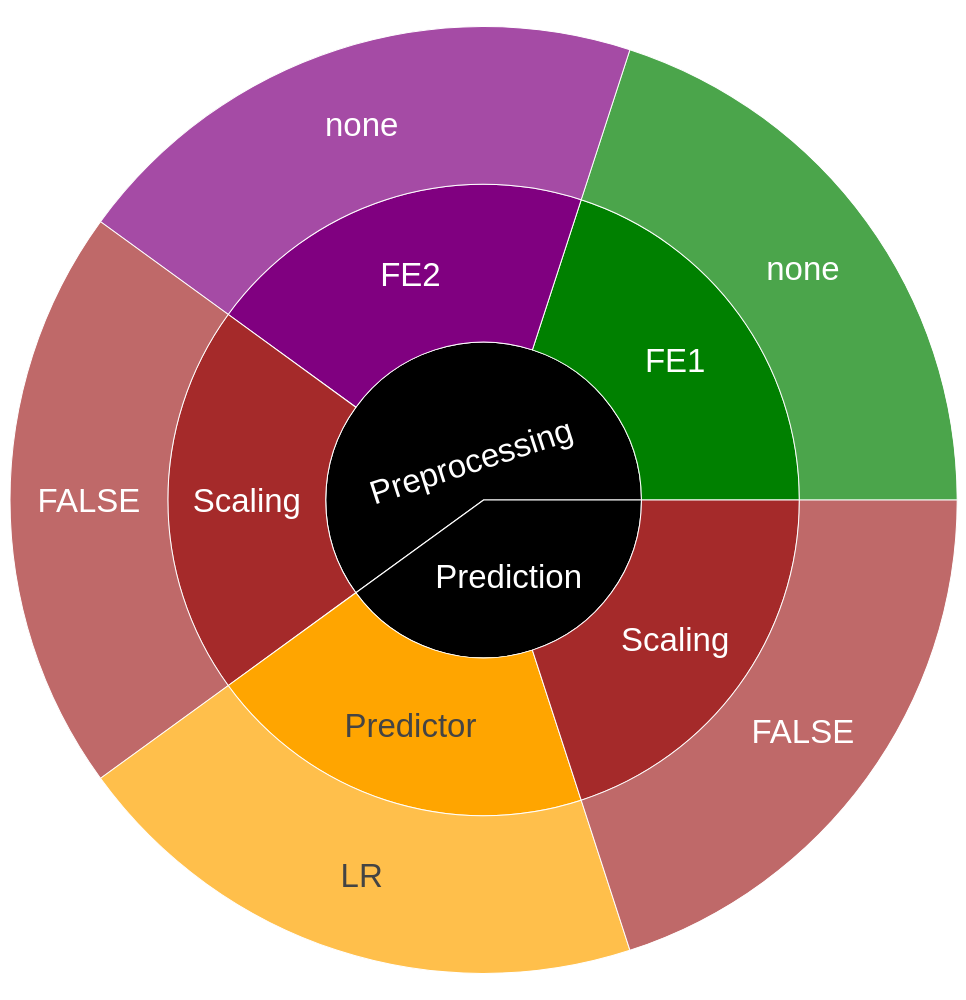
\includegraphics[width=0.9\textwidth]{img/sunburst/agnews.png}
    \caption{AGNews}
  	\end{subfigure}

  	\begin{subfigure}[t]{0.3\textwidth}
    \centering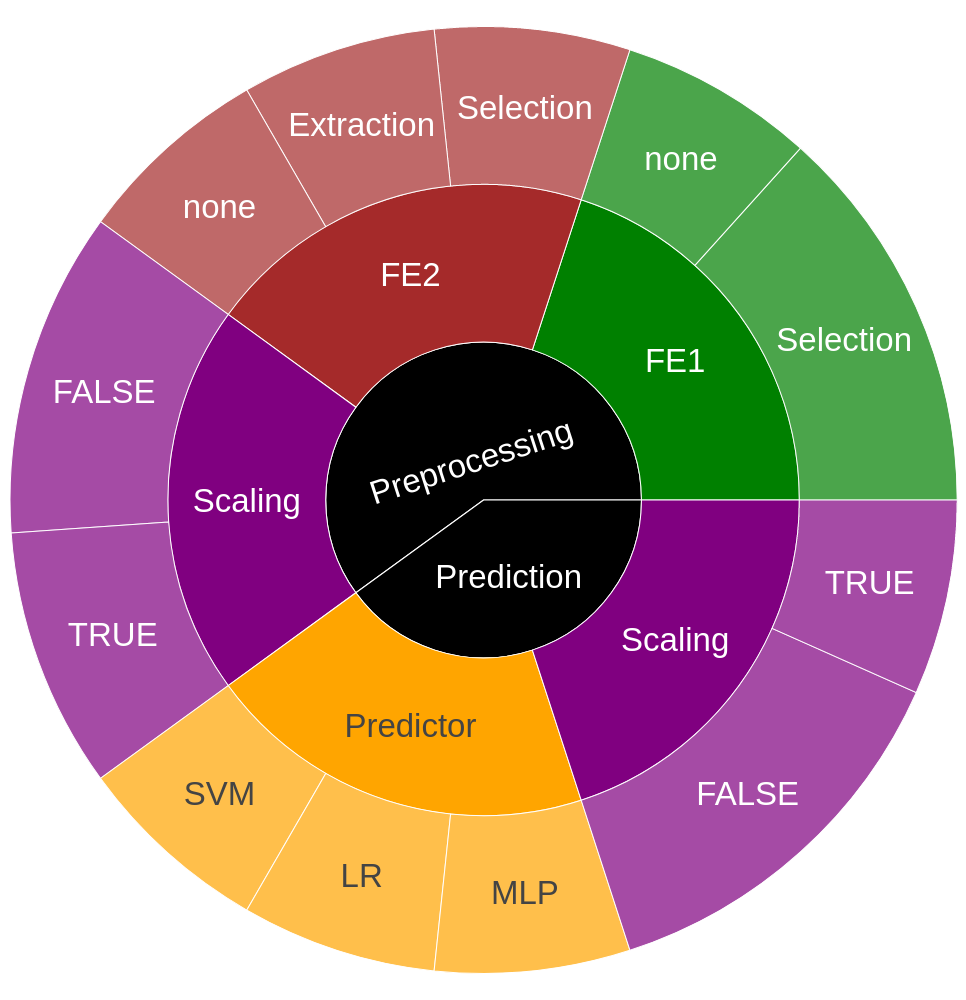
\includegraphics[width=0.9\textwidth]{img/sunburst/natal.png}
    \caption{Natal}
  	\end{subfigure}
	\begin{subfigure}[t]{0.3\textwidth}
    \centering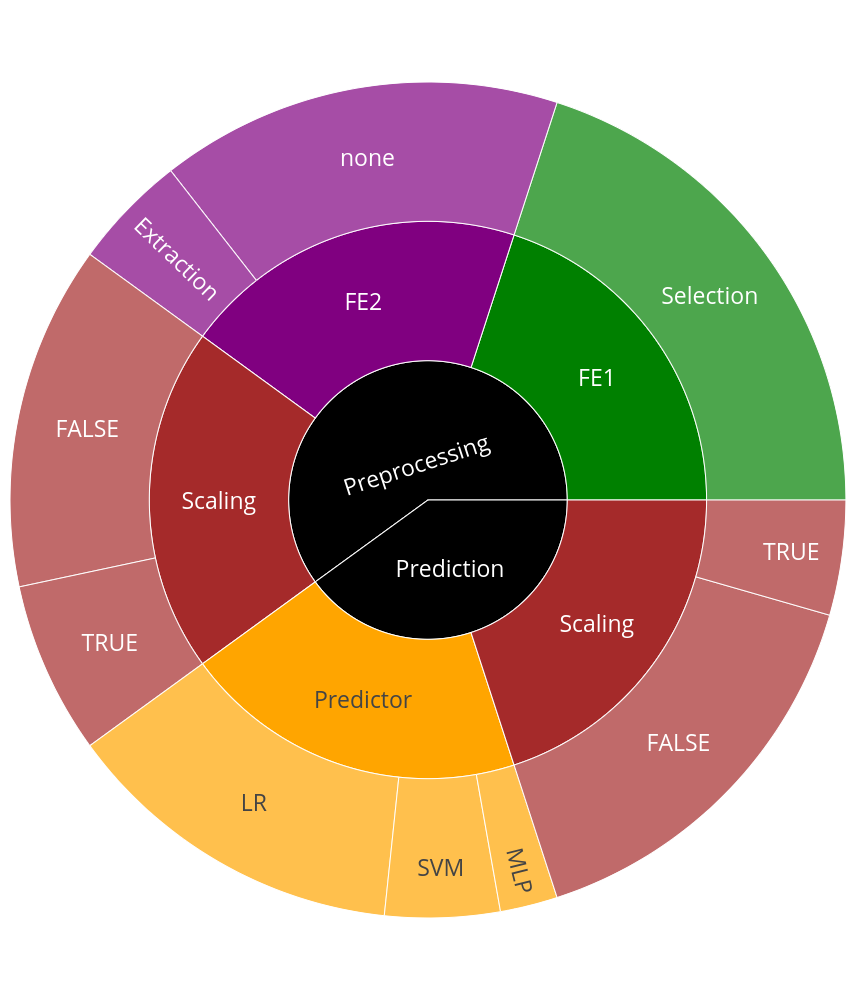
\includegraphics[width=0.9\textwidth]{img/sunburst/boston.png}
    \caption{Boston}
  	\end{subfigure}

    \caption{Pipeline composition for each dataset.}
    \label{fig:dataset_composition}
\end{figure*}